%
\documentclass[Proceedings]{ascelike}
%
% Feb. 14, 2013
%
% Some useful packages...
%
%\usepackage{graphicx}
%\usepackage{subfigure}
%\usepackage{amsmath}
%\usepackage{amsfonts}
%\usepackage{amssymb}
%\usepackage{amsbsy}
%\usepackage{times}
%
% \usepackage{float}
\usepackage{amsmath}
 \usepackage{graphicx}
 \usepackage{multirow}
 \usepackage{natbib}
% \usepackage{amssymb}
% \usepackage{amsthm}
 \usepackage{threeparttable}
%\usepackage{natbib}
\newtheorem{thm}{Theorem}
% Place hyperlinks within the pdf file (works only with pdflatex, not latex)
% \usepackage[colorlinks=true,citecolor=red,linkcolor=black]{hyperref}
%
%
% NOTE: Don't include the \NameTag{<your name>} if you have selected 
%       the NoPageNumbers option: this leads to an inconsistency and
%       a warning, and the NameTag is ignored.
% \NameTag{Kuhn, Feb. 14, 2013}
%
%
\begin{document}
%
% You will need to make the title all-caps
\title{Order-Constrained Reference Priors with
Implications for Analysis of Variance/Covariance Models}
%
\author{
% Maozhe Gong,\ Michael Sonksen,\ Gabriel Huerta%
%
% ---- The first of two styles for addresses: using footnotes and \thanks ----
% \thanks{
% Dept.\ of Civil Engrg.,
% Donald P.\ Shiley School of Engrg., Univ.\ of Portland, 
% 5000 N.\ Willamette Blvd.,
% Portland, OR  97203. E-mail: kuhn@up.edu.},
% \ Member, ASCE
%
% Adding a second author with the same affiliation (still using \thanks):
%  \\
%  Ima Colleague,\footnotemark[1] Member, ASCE%
%
% Adding another author with a different affiliation.  I have found that 
% the \and command doesn't quite work, so just use "and", as in the following 
% \\
% and
% Younyee Kuhn%
% \thanks{Flourishing wife of same.},%
% \ Not a Member, ASCE
%
% ---- The second of two styles for addresses: below names, no footnotes ----
%
% For this style, don't use \thanks.  Instead, use superscripts and carriage
% returns ("\\").  It's not pretty, but neither is the new ASCE proceedings
% style.  Something like the following:
%
% Matthew R. Kuhn$^1$, Member, ASCE\\[1ex]%
%
% $^1$\parbox[t]{5.75in}{Dept.\ of Civil Engrg.,
% Donald P.\ Shiley School of Engrg., Univ.\ of Portland, 
% 5000 N.\ Willamette Blvd., Portland, OR  97203. kuhn@up.edu.}
}
%
\maketitle
%
\begin{abstract}
Under the framework provided by \cite{BergerBernardo1992}, we proposed
theorems of deriving reference priors for Analysis of Variance (ANOVA)
and Analysis of Covariance models (ANCOVA) with a categorical variable
under common ordering constraints. The reference priors were further
investigated by simulation studies, with comparison to Jeffreys' prior
and Least Squares Estimation. Following that, we analyzed two data
sets: diabetes data in which the relationship between the type 2
diabetes risk (through Hemoglobin A1c) and different smoking levels is
studied and the rats data where the effect of d-amphetamine sulfate on
the behavior of rats was discussed. In both simulation studies and
real data set modeling, the reference priors incorporating the
internal order information showed good performances and were suggested
to use as default priors.
\end{abstract}
%
% Some keywords, using a new command: \KeyWords{}
%
\KeyWords{Reference priors, ANOVA/ANCOVA models, Ordering constraint.}
%


%Initially, I was working with my thesis advisor, Professor Mario
%Peruggia, on extending the Artificial Autoregressive Diagnostic (AAR)
%to non-normal models and we came across an interesting mortality rate
%dataset which had a poorly specified noninformative prior
%distribution.
%While in the process of developing a model diagnostic 
%for that model, we decided to find an appropriate
%noninformative prior distribution for the model. 
\section{1. Introduction}
The prior distribution plays a central role in Bayesian analysis and
statisticians spend a considerable amount of time looking for \emph{a
  prior} that suits their needs (subjective, objective, or other). In
real data analysis, a common situation is that the data analyst has
some known \emph{a priori} information about the parameters. For
example, in many applications inequality constraints among parameters
$\theta_i$, $i = 1, 2, ..., k$, may be adopted. Some common ordering
restrictions of interest are:\\

Simple order
\begin{eqnarray}
\theta_1<\theta_2<...<\theta_k\nonumber
\end{eqnarray}

Simple tree order
\begin{eqnarray}
\theta_1<\theta_i,\;i=2,...k\nonumber
\end{eqnarray}

Umbrella order(with peak at $i$)
\begin{eqnarray}
\theta_1<\theta_2<...<\theta_i>\theta_{i+1}...>\theta_k\nonumber
\end{eqnarray}
% it is not obvious how to turn this into a prior distribution. 
% when estimating the components of the parameter \pmb{${\mu}$} = ($\mu_1,\mu_2,...,\mu_k$)$^\prime$, if $\mu_i$ is the average height of US children of age i, then it is reasonable to assume the simple ordering, i.e,
% \begin{eqnarray}
% \mu_1<\mu_2<...<\mu_k
% \end{eqnarray}
% 

One example, explored by \cite{McDermott}, concerns patient outcomes
and drug dosages. It may be known that the effect of the placebo is
lower than any effects corresponding to dosage amounts of a drug
(simple tree order). Another reasonable assumption is that higher
dosages correspond to a larger effect(simple order). Incorporating
this information into a prior distribution is extremely attractive as
it can produce better inferences for the parameters, especially when
the sample size is small and variability of the data is large.

When posed with this information, the statistician must somehow
incorporate it into a functional form of a prior. One option is to
pick a subjective prior (perhaps conjugate to ease the derivation) and
simply add the ordering restrictions. However, unless care is taken in
the subjective prior elicitation that resulting prior may be much more
influential than originally envisioned. A similar problem can occur
when the constraints are naively applied to a standard non-informative
prior. In this work we utilize the reference prior framework of
\cite{BergerBernardo1992} to construct reference priors conditional on
these orderings. The derivation of the reference priors involves the
typical sequential maximization of the Kullback-Leibler divergence
between the prior and the posterior, which utilizes an iterative
algorithm and requires model parameters to be grouped and ordered by
inferential importance. A reference prior is then derived for the
given likelihood, conditional on the specified grouping and ordering.

Under the constraints in (1), (2) and (3), we derived the general
forms of the reference priors for any ordering and grouping. This
result can be used whenever the likelihood is regular and there are
additional conditions on the Fisher information matrix. With those
reference priors, the resulting models are a compromise between using
the subjective information and letting the data drive the inferences.

The rest of the paper is organized as follows. In Section 2, we derive
and evaluate the performance of reference priors in a simulation
study, with comparisons to Jeffreys' prior and Least Squares
Estimation. In Section 3, with our reference priors, we fit a Bayesian
ANCOVA model for the diabetes data and an ANOVA model for the rats
data. In Section 4, we provide the final conclusions.

\section{2. Reference Priors Subject to Order Restrictions}
\subsection{2.1 Prior Derivation}
Let us assume we have a model $Y_{ij}=\theta_i + \varepsilon_{ij}$
with $\varepsilon_{ij}\overset{iid}{\sim}N(0,1)$ for $i = 1, 2,
\hdots, k$ and $j = 1, \hdots, n_i.$ Let \pmb{$\theta$} =
\{$\theta_1,\;\theta_2,\hdots,\;\theta_k$\} with \pmb{$\theta$} $\in$
$\Theta$ and the $\theta$'s follow a certain order. Setting the
variance equal to 1 does not lose generality for this problem.

To derive reference priors for this model, we rely on the sequential
algorithm of \cite{BergerBernardo1992}. Since $\Theta$ is noncompact,
a compact subset $\Theta^l$ is needed, where $l$ is any real number
that denotes the boundary of the compact subset. The elements of
\pmb{$\theta$} are first partitioned into $m$ groups and ordered by
relative inferential importance, which gives \pmb{$\theta$} =
($\pmb{\theta}_{(1)},\;\pmb{\theta}_{(2)},\hdots,\;\pmb{\theta}_{(m)}$). Suppose
that group $j$ contains $m_j$ elements, that is, {$\pmb\theta_{(j)}$}
= $(\theta_{j_1},\;\theta_{j_2},\hdots,\;\theta_{j_{m_j}})$. Actually,
the user is totally in control of the specific ordering and grouping,
which may have a noticeable influence on the resulting prior
distribution.

Paralleling the grouping and ordering that we have above, the Fisher
information matrix for this Gaussian likelihood can be written as
\begin{eqnarray}
I(\boldsymbol{\theta})=\textrm{diag}[h_1(\boldsymbol{\theta}),\;h_2(\boldsymbol{\theta}),\hdots,\;h_m(\boldsymbol{\theta})].
\nonumber
\end{eqnarray} 
with $h_j$(\pmb{$\theta$}) =
$\textrm{diag}[n,\;n,\hdots,\;n]_{m_j\times m_j}$. Let us define
$\pmb\theta_{(1:j)}$ =
($\pmb{\theta}_{(1)},\;\pmb{\theta}_{(2)},\hdots,\;\pmb{\theta}_{(j)}$). Because
our model is regular and the determinant of $h_j(\pmb\theta)$,
$|h_j(\pmb\theta)|$ = $n^{m_j}$, we can use the simplified expression
for the reference prior that is given in Lemma 1 of
\cite{BergerBernardo1992} and obtain
\begin{eqnarray}\label{eq:ref_l}
\pi^{l}(\boldsymbol{\theta})
& = &
\frac{\Pi_{j=1}^{m}|h_j(\boldsymbol{\theta})|^{1/2}}{\Pi_{j=1}^{m}\int_{\Theta^{l}\cap[\Theta_{j}|\Theta_{(1:(j-1))}]}|h_j(\boldsymbol{\theta})|^{1/2}d\boldsymbol{\theta_{(j)}}}I_{\Theta^{l}}(\boldsymbol{\theta}),\label{Lemma1}
\end{eqnarray}
where $[\Theta_{j}|\Theta_{(1:(j-1))}]$ is the parameter space of $\pmb\theta_{(j)}$ given $\pmb\theta_{(1:(j-1))}$.

To derive a general expression for the reference prior, we need to
determine the integrals in the denominator of Equation
\ref{eq:ref_l}. We define $\pmb\theta_{(1:j),\;k}$ to be the $k^{th}$
element of the vector $\pmb\theta_{(1:j)}$. The term
$|h_j(\boldsymbol{\theta})|^{1/2}$ can be canceled out from Equation
\ref{eq:ref_l} because it is only a function of $n$. Under regularity
conditions, if the Fisher information matrix of the model satisfies
Lemma 1 in \cite{BergerBernardo1992}, careful calculation can prove
the following innovative theorems:

\begin{thm}
\label{theorem1}
For a simple order, $\theta_1<\theta_2<\hdots<\theta_k$,
\begin{eqnarray}
\pi^{l}(\boldsymbol{\theta})
& \propto &
\frac{1}{\Pi_{j=2}^{m}(\gamma_j-\eta_j)^{m_j}}I_{\Theta^{l}}(\boldsymbol{\theta})\nonumber
\end{eqnarray}
\end{thm}
with
\begin{displaymath}
\gamma_{j+1} = \left\{
\begin{array}{lr}
\min\limits_{k}\{\boldsymbol{\theta}_{(1:j),\;k}:\boldsymbol{\theta}_{(1:j),\;k}>\max[\boldsymbol{\theta}_{(j+1)}]\} &,\; if\; \max[\boldsymbol{\theta}_{(1:j)}]> \max[\boldsymbol{\theta}_{(j+1)}]\\
l &,\; if\; \max[\boldsymbol{\theta}_{(1:j)}]< \max[\boldsymbol{\theta}_{(j+1)}]
\end{array}
\right.
\end{displaymath} 
and
\begin{displaymath}
\eta_{j+1} = \left\{
\begin{array}{lr}
\max\limits_{k}\{\boldsymbol{\theta}_{(1:j),\;k}:\boldsymbol{\theta}_{(1:j),\;k}<\min[\boldsymbol{\theta}_{(j+1)}]\} &,\; if\; \min[\boldsymbol{\theta}_{(1:j)}]< \min[\boldsymbol{\theta}_{(j+1)}]\\
-l &,\; if\; \min[\boldsymbol{\theta}_{(1:j)}]> \min[\boldsymbol{\theta}_{(j+1)}].
\end{array}
\right.
\end{displaymath} 
%theorem 2
\begin{thm}
\label{theorem2}
For a simple tree order, $\theta_1<\theta_i,\ i=2,\hdots,k$,
\begin{eqnarray}
\pi(\boldsymbol{\theta})
& \propto &
I_{(\theta_1<\theta_i)}.\nonumber
\end{eqnarray}
\end{thm}
%theorem 3
\begin{thm} 
\label{theorem3}
For an umbrella order,
$\theta_1<\theta_2<\hdots<\theta_i>\theta_{i+1}>\hdots>\theta_k$,
parameters in group $j$ can be separately treated as (1) with
increasing order and (2) with decreasing order, then,
\begin{eqnarray}
\pi^{l}(\boldsymbol{\theta}) & \propto &
\frac{1}{\Pi_{j=2}^{m}(\gamma_{j1}-\eta_{j1})^{m_{j1}}(\gamma_{j2}-\eta_{j2})^{m_{j2}}}I_{\Theta^{l}}(\boldsymbol{\theta}).\nonumber
\end{eqnarray}
\end{thm}
$\gamma_{j1}$, $\eta_{j1}$, $\gamma_{j2}$ and $\eta_{j2}$ can be
determined by the definitions in Theorem \ref{theorem1} with
$m_{j1}+m_{j2}=m_j$. The final reference priors in the true parameter
space in Theorems \ref{theorem1} and \ref{theorem3} can be obtained by
making $l\to\infty$.

Detailed proofs can be found in the appendix. 

These three theorems are extension of the results in
\cite{Sonksen2012}. The theorems provide the general expressions that
can be used to determine the reference priors of any grouping and
ordering. In addition, if the variance $\sigma^2$ is introduced in the
model, it can be grouped by itself and considered as the first
grouping. Then the theorems derived above can be adopted without any
adjustment.


Further more, in more complicated models, such as a regression model
with a grouping variable of interest and other predictors, with the
same assumption that
$\varepsilon_{ij}\overset{iid}{\sim}N(0,\sigma^2)$, one can show that
the general expressions of the reference priors, given the mean
responses of the grouping variable follow a common order, share the
same forms as we showed in Theorem \ref{theorem1}, Theorem
\ref{theorem2} and Theorem \ref{theorem3}.
\subsection{2.2 Simulation Study}
In this simulation study, we focus on a one-way ANOVA model with group
means following a simple order, i.e., $\mu_1<\mu_2<\hdots<\mu_k$. To
derive the reference priors for this model, the user has to specify
the ordering and grouping of the parameters. \cite{BergerBernardo1992}
suggest to completely separate the parameters with groups of one
element each. On the other hand, \cite{Sonksen2012} follow the
\cite{NichollsJones} approach and suggest that the primary attention
should be given to the extreme parameters, i.e., $\mu_1$ and
$\mu_k$. Based on the general expression derived in Theorem
\ref{theorem1}, we consider these two ways of grouping and ordering
and label them as $\pi(\pmb\theta)_{uni}$ and $\pi(\pmb\theta)_{u1k}$,
respectively. The resulting prior distributions are listed in Table
\ref{tab:ref}.
\begin{table}[h!]
\centering
\begin{threeparttable}
\caption{Reference priors for one-way ANOVA model with a simple order}
\begin{tabular}{c|c|c}
\multirow{1}{*}{Label}&Parameter Grouping and Ordering&Reference
Prior\\ \hline
\multirow{1}{*}{$\pi(\pmb\theta)_{uni}$}&$(\{\sigma^2\}, \{\mu_1\},
\hdots, \{\mu_k\})$&$\frac{1}{\sigma^2}\times
I_{\Theta}(\boldsymbol{\theta})$\\ \multirow{1}{*}{$\pi(\pmb\theta)_{u1k}$}&$(\{\sigma^2\}$,
$\{\mu_1,\;\mu_k\}$, $\{\mu_2,\; \hdots,\;
\mu_{k-1}\})$&$\frac{1}{\sigma^2}\times\frac{1}{{(\mu_k-\mu_1)}^{k-2}}\times
I_{\Theta}(\boldsymbol{\theta})$
\end{tabular}
\begin{tablenotes}
\item Note: $\pmb\theta$ = $\{\pmb\beta,\;\sigma^2\}$ = $\{\mu_1,\hdots,\mu_k,\;\sigma^2\}$. $\Theta$ = $\{(\pmb\beta,\sigma^2) : -\infty<\mu_1<\hdots<\mu_k< +\infty $ and $0<\sigma^2< +\infty \}$.
\end{tablenotes}
\label{tab:ref}
\end{threeparttable}
\end{table}

The total number of simulated studies is 1000. Each study is analyzed
by obtaining 11000 MCMC iterations and the first 1000 iterations are
treated as burn-in. With an acceptance rate around 0.4, the posterior
medians are used as the Bayesian estimates.

For each setting, the 95\% credible or confidence intervals are
determined and the true parameter values are checked to see if covered
by the 95\% intervals for each method. The empirical coverages of the
intervals are then computed based on these 1000 simulations. The root
mean square error (RMSE) for each parameter between estimates and real
parameter value is also calculated. The average DIC from simulations
is determined for each prior as an important tool for Bayesian model
comparison and selection. The detailed settings and results are shown
in the following figures and later discussed in detail.

\begin{figure}[h!]
\centering
\resizebox{1\textwidth}{!}{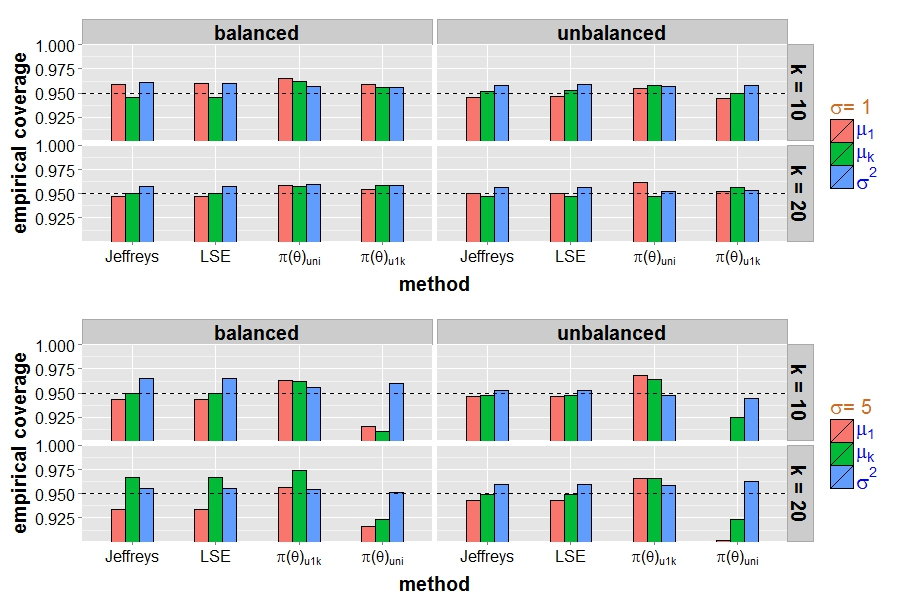
\includegraphics{pic/anova_coverage.jpeg}}
\caption{Empirical coverage of 95\% CI under different settings and methods.}
\label{fig:anova_coverage}
\end{figure}

\begin{figure}[h!]
\centering
\resizebox{1\textwidth}{!}{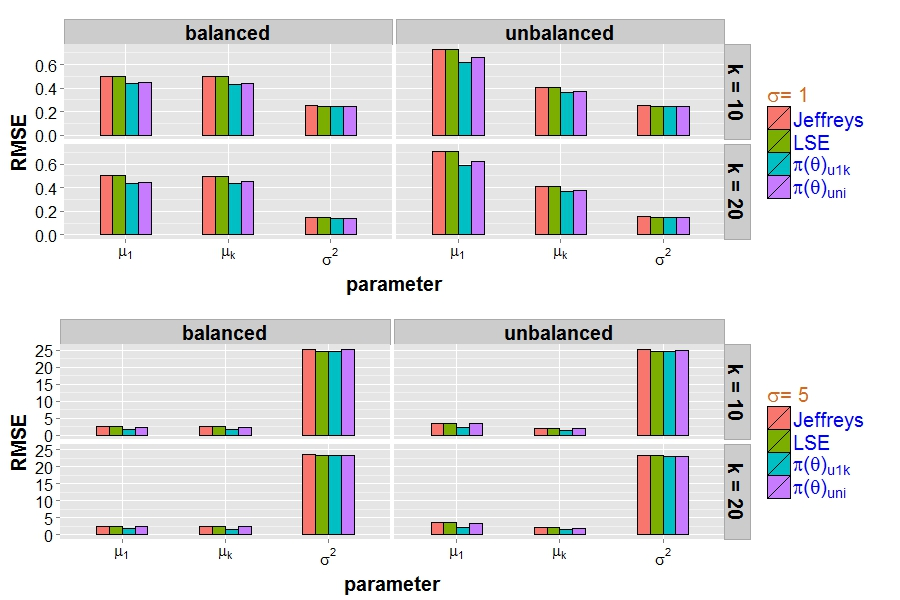
\includegraphics{pic/anova_rmse.jpeg}}
\caption{RMSE comparisons of $\mu_1$, $\mu_k$ and $\sigma^2$ under different settings and methods.}
\label{fig:anova_rmse}
\end{figure}
\begin{figure}[h!]
\centering
\resizebox{.6\textwidth}{!}{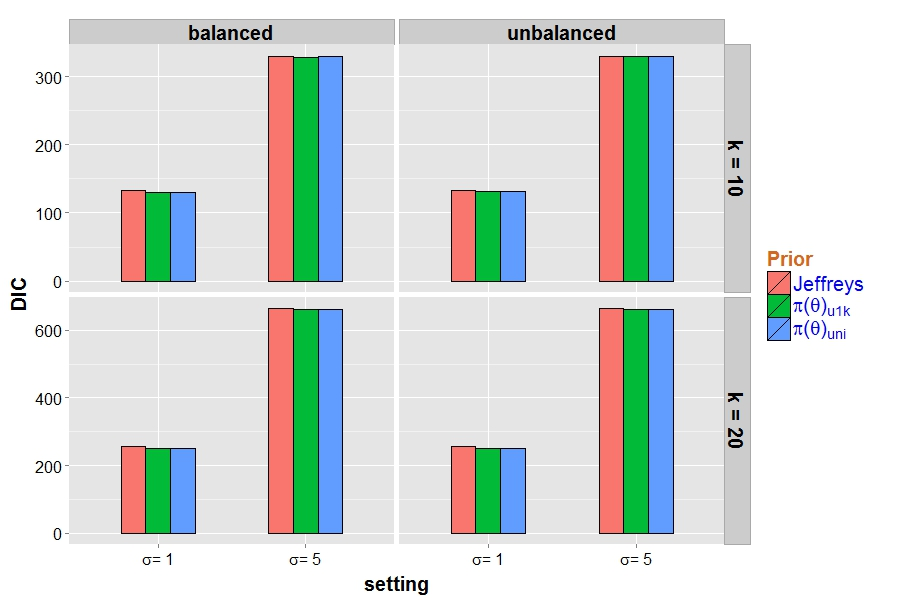
\includegraphics{pic/ANOVA_DIC.jpeg}}
\caption{Average DIC comparisons of three Bayesian methods.}
\label{fig:DIC_ano}
\end{figure}


All the simulation results from 8 different settings are summarized in
Figures \ref{fig:anova_coverage}-\ref{fig:DIC_ano} for $k$ = 10 or 20,
$\sigma$ = 1, 5 and $n$ = 40, 80. Figure \ref{fig:anova_coverage}
shows the empirical coverages of 95\% confidence or credible
intervals. All these coverages look close to 0.95 except when $\sigma$
= 5, the coverage of $\pi(\pmb\theta)_{uni}$ is relatively low
especially for unbalanced design. This is in accordance with the fact
that when the variance is large, the estimates from
$\pi(\pmb\theta)_{uni}$ are somewhat off the true values for $\mu_1$
and $\mu_k$.

Figure \ref{fig:anova_rmse} shows the RMSEs of $\mu_1$, $\mu_k$ and
$\sigma^2$ under different settings. The reference prior
$\pi(\pmb\theta)_{u1k}$ always gives the smallest RMSE when estimating
$\sigma^2$, although the RMSEs from these four methods are actually
close. When estimating $\mu_1$ and $\mu_k$, the reference prior
$\pi(\pmb\theta)_{u1k}$ tends to give the smallest RMSE under all
settings. The reference prior $\pi(\pmb\theta)_{uni}$ also gives
pretty small RMSEs when $\sigma$ = 1, however, this is not obvious
when $\sigma$ = 5.

Figure \ref{fig:DIC_ano} shows simulation averages for DIC under the
three Bayesian priors. The resulting values are close and the
reference prior $\pi(\pmb\theta)_{u1k}$ always gives the smallest
average DIC value while Jeffreys' prior seems the worst.

Based on all our simulation results, we can conclude the reference
priors that consider the internal order information are good choices
when dealing with isotonic models, especially when the number of
parameters is large. Under this situation the internal ordering
information is important and the reference priors that incorporates
this information stand out and work really well when looking for
default priors.
\section{3. Application of Reference Priors}
\subsection{Smoking and Type 2 Diabetes}
In 2013, Dr.\ Mark Burge at UNM Health Science Center started a study
with regard to type 2 diabetes. In this study, 218 adults in New
Mexico at risk for type 2 diabetes were screened to determine their
glucose homeostasis status. Hemoglobin A1c (HbA1c), a common variable
used to measure diabetes status, was measured for each patient along
with other variables, such as the participant's high-density
lipoprotein (HDL), body mass index (BMI) and age etc. \\
\begin{figure}[h!]
\centering
\resizebox{1\textwidth}{!}{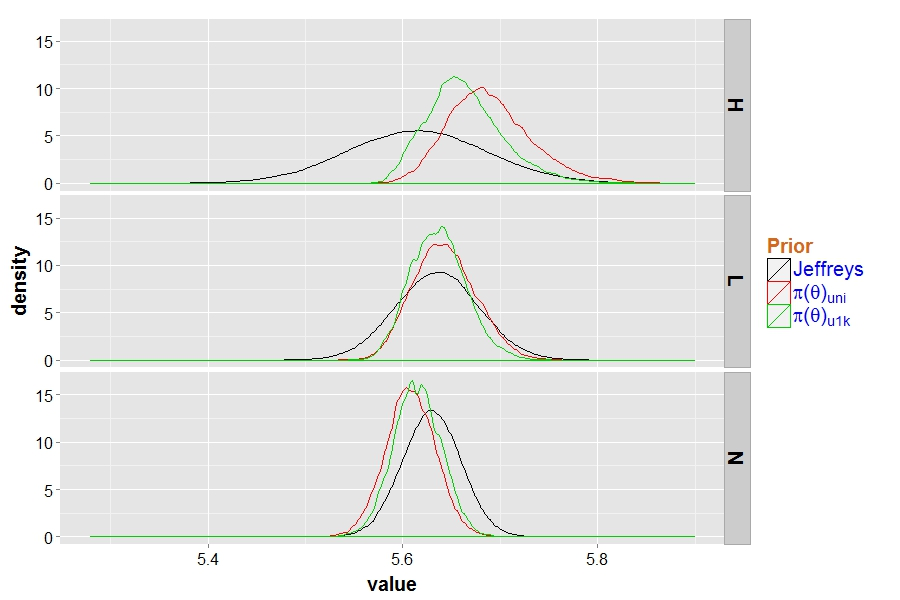
\includegraphics{pic/HbA1c_density.jpeg}}
\caption{Marginal posterior distributions for different smoking levels under three priors}
\label{fig:HbA1c2}
\end{figure}
Among these potential covariates the smoking levels become interesting
in that: Smoking tends to induce high risk of having type 2 diabetes
\citep{smoking}. At the same time, people with diabetes who smoke are
more likely than nonsmokers to have trouble with insulin
dosing. However, this relationship sometimes is masked by the
variability in observational data. That is, smoking may show a
non-significant effect, which will certainly hamper the interpretation
of the model. In this section, we assume internal order information
and that there is a simple order for the mean responses of smoking
levels. Then, we construct an ANCOVA model to investigate the
relationship of type 2 diabetes and smoking along with several other
covariates. We adopt the reference priors derived in previous sections
and perform an analysis under a Bayesian framework. For comparisons,
we also consider Jeffreys' prior and LSE approaches. We use three
classifications for smoker status: High-level smokers (more than 10
pack-years), Low-level smokers (between 0 and 10 pack years) and
non-smokers (0 pack years), or H, L, N. Variable selection is done by
classical regression and LDL, BMI and ages of the participants seem
important for the model. After centering these variables, we add the
smoking effect, which contains three levels: High, Low and None.\\
\begin{table}[h!]
  \centering
  \caption{Bayesian analysis for diabetes data with reference priors and Jeffreys' prior}
\begin{tabular}{|l|c|c|c|c|c|c|c|c|c|}
    \hline
Smoking & \multicolumn{3}{|c|}{$\pi(\pmb\theta)_{u1k}$} &\multicolumn{3}{|c|}{$\pi(\pmb\theta)_{uni}$}&\multicolumn{3}{|c|}{Jeffreys}\\
\cline{2-10}
level & 2.5\% & mean & 97.5\% & 2.5\% & mean & 97.5\% & 2.5\% & mean & 97.5\%  \\
\hline
N & 5.557 & 5.609 &  5.658 & 5.556 & 5.608 &  5.661 & 5.574 & 5.630 & 5.692 \\
L & 5.588 & 5.645 & 5.708 & 5.584 & 5.643 & 5.710 & 5.552 & 5.636 &  5.718  \\
H & 5.619 & 5.692 & 5.785 & 5.619 & 5.692 & 5.787 & 5.473 & 5.618 & 5.771  \\
\hline
DIC& \multicolumn{3}{|c|}{1513} &\multicolumn{3}{|c|}{1532}&\multicolumn{3}{|c|}{1542}\\
\hline
\end{tabular}
\label{tab:mcmc}
\end{table}

A Bayesian analysis with a prior distribution that considers a simple
order for the smoking effects can be performed, where heavier smokers
induce higher risk of type 2 diabetes. Two reference priors,
$\pi(\pmb\theta)_{uni}$ and $\pi(\pmb\theta)_{u1k}$ are
considered. Fitted models can be compared with Jeffreys' prior
$\pi(\pmb\theta)_{J}\propto \frac{1}{\sigma^2}$. Figures
\ref{fig:HbA1c2} shows the marginal posterior distributions of the
mean responses of different smoking levels under the different
priors. Posterior distributions from two reference priors show similar
patterns, which is not surprising since the sample size is fairly
large. The results from Jeffreys' prior are close to LSE, where the
estimates for the three smoking levels tend to be mixed up. Compared
with the reference priors, the marginal posterior from Jeffreys' prior
seems to have heavier tail when estimating the mean responses for
different smoking levels (Figure \ref{fig:HbA1c2}), while they behave
similarly when estimating other parameters.

The MCMC results based on different priors is summarized in Table
\ref{tab:mcmc}. Although Jeffreys' prior gives similar results as
classical regression, its DIC is the largest. The one with the
reference prior $\pi(\pmb\theta)_{u1k}$ gives the smallest DIC, which
turns to be the evidence of better fitting and less complexity of the
model. If we consider the differences between different smoking
levels, the reference priors incorporating the simple order show there
is a significant difference between high level smokers and
non-smokers, while the results from Jeffreys' prior cannot show this
relationship.

\subsection{Rats and d-Amphetamine
Sulfate} In \cite{Heffner1974}, the effect of d-amphetamine sulfate on
the behavior of rats was discussed , where the lever press rate at
which a rat deprived of water pressed a lever to get water was
considered. The rate was defined as the total number of lever pressed
divided by the elapsed time (in seconds) during a session for a given
dosage of amphetamine. The resulting data show that the dose-response
relationship has a downturn at high dosages. Other studies, such as
\cite{Dews1958}, where the relationship between amphetamine and key
pecking by pigeons was studied, also show a similar pattern. It is
reasonable to anticipate the effect of d-amphetamine sulfate on a
rat's rate of lever pressing follows an umbrella order. That is, the
initial rate increases as the drug dosage increases and decreases at
high dosages.
\begin{table}[h!]
  \centering
  \caption{d-Amphetamine sulfate dosage and rats}
\begin{tabular}{|l|c|c|c|c|c|}
    \hline
 & \multicolumn{5}{|c|}{Dosage (mg/kg)}   \\

\cline{2-6}
Rats & 0.0 &0.5 & 1.0 & 1.5 & 2.0 \\
\hline
1   &0.60 	&0.80 	&0.82 	&0.81 	&0.50\\
2 	&0.51 	&0.61 	&0.79 	&0.78 	&0.77\\
3 	&0.62 	&0.82 	&0.83 	&0.80 	&0.52\\
4 	&0.60 	&0.95 	&0.91 	&0.95 	&0.70\\
5 	&0.92 	&0.82 	&1.04 	&1.13 	&1.03\\
6 	&0.63 	&0.93 	&1.02 	&0.96 	&0.63\\
7 	&0.84 	&0.74 	&0.98 	&0.98 	&1.00\\
8 	&0.96 	&1.24 	&1.27 	&1.20 	&1.06\\
9 	&1.01 	&1.23 	&1.30 	&1.25 	&1.24\\
10 	&0.95 	&1.20 	&1.18 	&1.23 	&1.05\\
\hline
\end{tabular}
  \label{tab:rats}
\end{table}
As shown in Table \ref{tab:rats}, we adopt this data as another
example for our reference priors. In this data, ten male albino rats
of the same strain and of approximately the same weight were
included. The study contains five dosage levels of the drug, including
a zero level of a saline solution. Each rat received all five dosage
levels randomly. One hour after a drug injection, an experimental
session started during which the rat received water each time after a
second lever was pressed. If each rat is treated as a block and the
focus of the analysis is on the treatments, i.e., different dosage
levels, then a randomized block design ANOVA model can be set up as:

\begin{eqnarray}
  \pmb{y}
    & = &
X\pmb{\theta}+\pmb{\varepsilon},\; \pmb{\varepsilon}{\sim}N(\pmb{0},\sigma^2 I),
\nonumber
\end{eqnarray}
, where ${\boldsymbol\theta}=(\tau_1,...\tau_5,\beta_2,...\beta_{10})^\prime$. $\tau$ stands for treatment effect and $\beta$ stands for block effect.
Based on \cite{Mack1981} and \cite{Lim1997}, we can estimate the peak of treatment effect at $\hat{p}$=3, 1.0 mg/kg dosage. One way to group and order the parameters is:
$(\{\sigma^2\}$, $\{\tau_1,\;\tau_3\}$, $\{\tau_4,\; \tau_5\}$,$\{\tau_2\})$,$\{\boldsymbol\beta\})$. Based on theorem 3, we can derive the corresponding reference prior, which is $\frac{1}{\sigma^2} \times \frac{1}{\tau_3-\tau_5} \times \frac{1}{\tau_3-\tau_1}\times I_{\Theta}(\boldsymbol{\theta})$.

\begin{figure}[h!]
\centering
\resizebox{1\textwidth}{!}{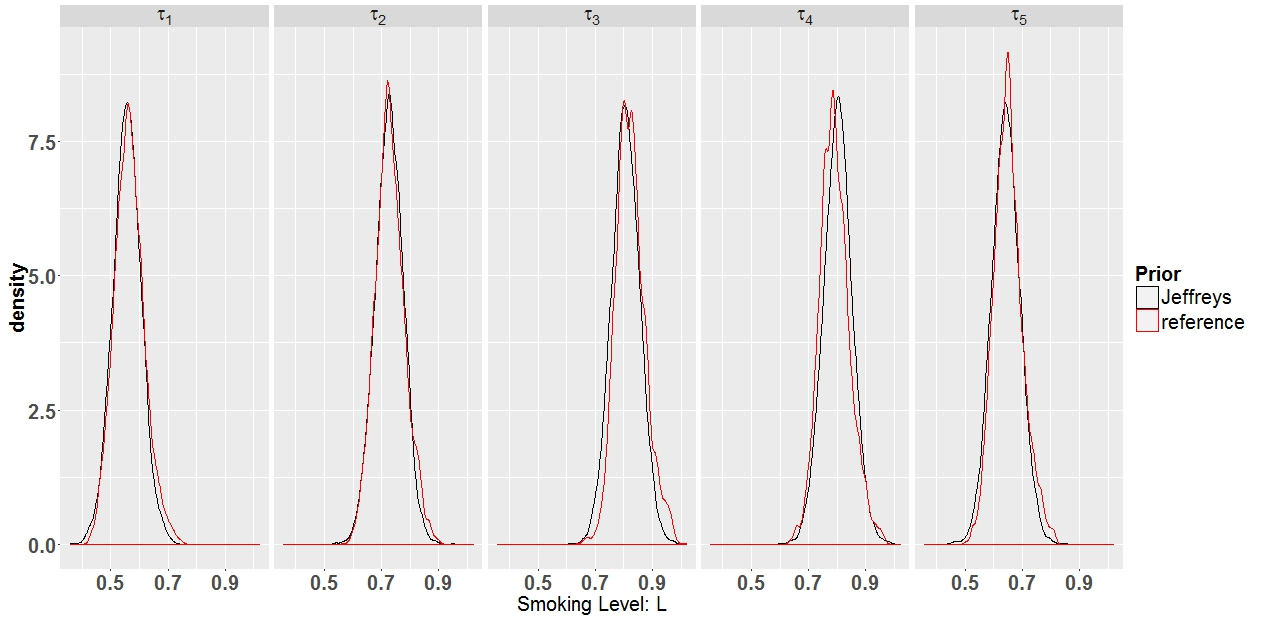
\includegraphics{pic/rats_mp.jpeg}}
\caption{Marginal posterior distributions for treatment effects under different dosage levels}
\label{fig:rats}
\end{figure}
We fit the above ANOVA model with this reference prior and Jeffreys' prior. The marginal posterior distributions for 5 treatment effects are shown in Figure \ref{fig:rats} and the major results are summarized in Table \ref{tab:rat_mcmc}. As shown in the figure and table, although the model fittings from the two priors are very similar, the model with the reference prior where the umbrella order is considered provides a more reasonable inference. It highlights the peak in the treatments groups, which can be very important especially when this relationship is masked by the variability of the data.
\begin{table}[h!]
  \centering
  \caption{Bayesian analysis for rats data with reference priors and Jeffreys' prior}
\begin{tabular}{|l|c|c|c|c|c|c|}
    \hline
Dosage &\multicolumn{3}{|c|}{reference}&\multicolumn{3}{|c|}{Jeffreys}\\
\cline{2-7}
level & 2.5\% & mean & 97.5\% & 2.5\% & mean & 97.5\%  \\
\hline
$\tau_1$ & 0.466 & 0.564 &  0.677 & 0.457 & 0.556 &  0.656 \\
$\tau_2$ & 0.632 & 0.729 & 0.838 & 0.629 & 0.727 & 0.821   \\
$\tau_3$ & 0.733 & 0.823 & 0.942 & 0.708 & 0.806 & 0.903  \\
$\tau_4$ & 0.694 & 0.791 & 0.904 & 0.701 & 0.802 & 0.901  \\
$\tau_5$ & 0.560 & 0.651 & 0.765 & 0.545 & 0.643 & 0.742  \\
\hline
DIC& \multicolumn{3}{|c|}{8173} &\multicolumn{3}{|c|}{8217}\\
\hline
\end{tabular}
\label{tab:rat_mcmc}
\end{table}

\section{4. Conclusions}
Under the frame-work by \cite{BergerBernardo1992}, we provide the
general formulas of the reference priors for ANOVA and ANCOVA models
with a categorical variable under common ordering constraints. The
derivation is a compromise of subjective information and ``let the
data talk itself''. Both simulation studies and data analysis suggests
incorporating the ordering information can improve goodness-of-fit,
which can be adopted as typical priors when handling similar
questions.

The three common ordering restrictions summarized at the beginning
cover the most common types of multiple comparisons for dose-finding
studies. The proposing method could be broadly used in modeling
dose-response relationship, for both monotonous relationship and
``inverted U-shape'' pattern. They can be treated as candidate models
in Multiple Comparison Procedures - Modelling (MCP-Mod) methodology,
where a ``best'' model can be selected through optimal model contrasts
while controlling the family-wise error rate by the use of multiple
comparison procedures. An optimal dose can then be determined
afterwards.

\pagebreak
%
%
% Now we start the appendices, with the new section name, "Appendix", and a 
%  new counter, "I", "II", etc.
%
\section*{Appendix}

\subsection*{Proof of Theorem 1}

\begin{eqnarray*}
\pi(\boldsymbol{\theta}) &\propto& \frac{1}{\prod_{j=2}^{m}\left(\gamma_j - \nu_j\right)^{m_j}} \label{thm1}
\end{eqnarray*}

Above it was shown that $|h_j(\boldsymbol{\theta})|=n^{m_j}$ thus the
numerator of Equation~\cite{Lemma1} is a constant.
% Sort out the parameter space.

% Describe the integral
% Take limits. 

The anti-derivative $\int |h_j(\boldsymbol{\theta})|^{1/2} d\theta = n^{m_j/2}\theta$. 





\[
\Theta^l = \left\{ \boldsymbol{\theta} : -l < \theta_1 <\theta_2 < \ldots < \theta_k < l \right\}
\]



\[
\int d\boldsymbol{\theta}_{(j)}
\]





\subsection*{Works Cited}\label{section:references}
%
% Here's the first appendix, the list of references:
%
\bibliography{research}
%
% And now for some pretty impressive notation.  In this example, I have used
%   the tabular environment to line up the columns in ASCE style.
%   Note that this and all appendices (except the references) start with 
%   the \section command
%
% \section{Notation}
% \emph{The following symbols are used in this paper:}%\par\vspace{0.10in}
% \nopagebreak
% \par
% \begin{tabular}{r  @{\hspace{1em}=\hspace{1em}}  l}
% $D$                    & pile diameter (m); \\
% $R$                    & distance (m);      and\\
% $C_{\mathrm{Oh\;no!}}$ & fudge factor.
% \end{tabular}
%

\end{document}
